\documentclass[answers]{exam}\newcommand{\repositoryInformationSetup}{     \usepackage[dvipsnames]{xcolor}     \usepackage[ angle=90, color=black, opacity=1, scale=2, ]{background}      \SetBgPosition{current page.west}      \SetBgVshift{-4.5mm}      \backgroundsetup{contents={{\color{green}\texttt{-{}-} differs from commit \texttt{f3526e2} in 0 files}}} } \newcommand{\commit}{{{\color{green}f3526e2}}}\usepackage{amsmath}
\usepackage{xspace}
\usepackage{bbm}
\usepackage{ifthen}



\newcommand{\repoURL}{https://github.com/evanberkowitz/umd-phys-373}



\newcommand{\secref}[1]{Sec.~\ref{sec:#1}}
\newcommand{\Secref}[1]{Section~\ref{sec:#1}}
\newcommand{\appref}[1]{App.~\ref{sec:#1}}
\newcommand{\Appref}[1]{Appendix~\ref{sec:#1}}
\newcommand{\tabref}[1]{Tab.~\ref{tab:#1}\xspace}
\newcommand{\Tabref}[1]{Table~\ref{tab:#1}\xspace}
\newcommand{\figref}[1]{Fig.~\ref{fig:#1}\xspace}
\newcommand{\Figref}[1]{Figure~\ref{fig:#1}\xspace}
\newcommand{\Eqref}[1]{Equation~\ref{eq:#1}\xspace}
\def\Ref#1{Ref.~\cite{#1}} \newcommand{\Reference}[1]{Reference~\cite{#1}}
\newcommand{\Refs}[1]{Refs.~\cite{#1}}
\newcommand{\References}[1]{References~\cite{#1}}



\newcommand{\issue}[1]{\href{\repoURL/issues/#1}{Issue #1}}
\newcommand{\pullrequest}[1]{\href{\repoURL/pulls/#1}{Pull Request #1}}



\newcommand{\arxiv}[1]{\href{http://www.arxiv.org/abs/#1}{arXiv:#1}}



\newcommand{\goesto}{\ensuremath{\rightarrow}}
\newcommand{\infinity}{\infty}
\newcommand{\Integers}{\mathbb{Z}\xspace}
\newcommand{\integers}{\Integers}
\newcommand{\one}{\ensuremath{\mathbbm{1}}}
\newcommand{\order}[1]{\ensuremath{\mathcal{O}\left(#1\right)}\xspace}
\newcommand{\Rationals}{\mathbb{Q}\xspace}
\newcommand{\Reals}{\mathbb{R}\xspace}
\newcommand{\Complexes}{\mathbb{C}\xspace}
\newcommand{\union}{\ensuremath{\cup}}
\DeclareMathOperator{\erf}{erf}
\newcommand{\laplace}[1]{\ensuremath{\mathcal{L}\left\{#1\right\}}\xspace}
\newcommand{\inverselaplace}[1]{\ensuremath{\mathcal{L}\inverse\left\{#1\right\}}\xspace}


\DeclareMathOperator{\odd}{odd}
\DeclareMathOperator{\even}{even}
\DeclareMathOperator{\sinc}{sinc}
\DeclareMathOperator{\real}{Re}
\DeclareMathOperator{\imag}{Im}





\DeclareMathOperator{\sech}{sech}
\DeclareMathOperator{\csch}{csch}
\DeclareMathOperator{\arccosh}{arccosh}
\DeclareMathOperator{\arcsinh}{arcsinh}
\DeclareMathOperator{\arctanh}{arctanh}
\DeclareMathOperator{\arcsech}{arcsech}
\DeclareMathOperator{\arccsch}{arccsch}
\DeclareMathOperator{\arccoth}{arccoth}



\DeclareMathOperator{\arcsec}{arcsec}
\DeclareMathOperator{\arccot}{arccot}
\DeclareMathOperator{\arccsc}{arccsc}



\newcommand{\oneover}[1]{\ensuremath{\frac{1}{#1}}}                             \newcommand{\inverse}{\ensuremath{^{-1}}}                                       \providecommand{\half}{\ensuremath{\frac{1}{2}} }                               \renewcommand{\half}{\ensuremath{\frac{1}{2}} }                                 \newcommand{\quarter}{\ensuremath{\frac{1}{4}} }                                



\newcommand{\dd}[3][1]{
    \ifthenelse { \equal {#1} {1} }
                {\ensuremath{\frac{d#2}{d#3}}}
                {\ensuremath{\frac{d^{#1}#2}{d#3^{#1}}}}
    }

\newcommand{\pp}[3][1]{
    \ifthenelse { \equal {#1} {1} }
                {\ensuremath{\frac{\partial#2}{\partial#3}}}
                {\ensuremath{\frac{\partial^{#1}#2}{\partial#3^{#1}}}}
    }

\newcommand{\ppp}[3]{\ensuremath{\frac{\partial^2#1}{\partial#2\,\partial#3}}}

\newcommand{\grad}{\ensuremath{\nabla}\xspace}
\newcommand{\laplacian}{\ensuremath{\grad^2}\xspace}

\providecommand{\id}{}
\renewcommand{\id}[1]{\ensuremath{\; \mathrm{d}#1}}

\newcommand{\abs}[1]{\ensuremath{\left| #1 \right|}\xspace}
\newcommand{\magnitude}{\abs}
\newcommand{\average}[1]{\ensuremath{\left\langle #1 \right\rangle}\xspace}

\newcommand{\ket}[1]{\ensuremath{\left|\;#1\;\right\rangle}}
\newcommand{\bra}[1]{\ensuremath{\left\langle\;#1\;\right|}}
\newcommand{\bracket}[2]{\ensuremath{\left\langle\;#1\;\middle|\;#2\;\right\rangle}}
\let\braket\bracket
\newcommand{\operator}[3]{\ensuremath{\left|\;#1\;\middle\rangle\; #2\; \middle\langle\;#3\;\right|}}



\newcommand{\identity}{\ensuremath{\mathds{1}}}
\newcommand{\diag}[1]{\ensuremath{\text{diag}\left(#1\right)}}
\newcommand{\tr}[1]{\ensuremath{\text{tr}\left[#1\right]}}
\newcommand{\transpose}{\ensuremath{{}^{\top}}}
\newcommand{\adjoint}{\ensuremath{{}^{\dagger}}}








\newcommand{\bash}{\texttt{bash}\xspace}
\newcommand{\git}{\texttt{git}\xspace}
\newcommand{\make}{\texttt{make}\xspace}
\newcommand{\mpi}{\texttt{MPI}\xspace}
\newcommand{\python}{\texttt{python}\xspace}

\let\builtinLaTeX\LaTeX
\def\LaTeX{\builtinLaTeX\xspace}
 \usepackage{amsmath,amssymb}
\usepackage{bm}
\usepackage{comment}
\usepackage{graphicx}
\usepackage[dvipsnames]{xcolor}
\usepackage{tikz}
\usepackage{tkz-euclide}
\usepackage{slashed}
\usepackage[
    colorlinks=true,
    allcolors=blue
]{hyperref}
\usepackage{tikz}
\usetikzlibrary{calc,patterns,decorations.pathmorphing,decorations.markings}
\usepackage{pgfplots}




\providecommand{\repositoryInformationSetup}{} \repositoryInformationSetup








\begin{document}

\title{Homework 12 --- PHYS373 2021}

\author{Douglas Domingues}

\date{Due May 13, 2021}

\maketitle

\begin{questions}

	\section*{PDEs}
	\question Boas 13.1.2a

	\begin{solution}
		``Show that the expression $u = \sin (x - vt)$ describing a sinusoidal wave (see Chapter 7, Figure 2.3), satisfies the wave equation (1.4)."
		Equation 1.4 is $$\laplacian u = \frac{1}{v^2} \frac{\partial^2u}{\partial t^2}$$

		$$ \laplacian \sin(x-vt) = -\sin(x-vt)$$
		$$ \frac{\partial^2}{\partial t^2} \sin(x-vt) = -v^2\sin(x-vt)$$
		$$ \frac{1}{v^2} \frac{\partial^2}{\partial t^2} \sin(x-vt) = -\sin(x-vt)$$
		Thus, indeed:
		$$ \laplacian \sin(x-vt) = \frac{1}{v^2} \frac{\partial^2}{\partial t^2} \sin(x-vt) $$

		``Show that, in general, $u = f (x - vt)$ and $u = f (x + vt)$ satisfy the wave equation, where $f$ is any
		function with a second derivative."

		Similarly to the first part,
		$$ \laplacian f(x-vt) = f''(x-vt)$$
		$$ \frac{\partial^2}{\partial t^2} f(x-vt) = v^2 f''(x-vt)$$
		$$ \frac{1}{v^2} \frac{\partial^2}{\partial t^2} f(x-vt) =  f''(x-vt)$$
		Therefore $f(x-vt)$ is a solution.

	\end{solution}
	\question Boas 13.2.3

	\begin{solution}
		``Solve the semi-infinite plate problem if the bottom edge of width $\pi$ is held at
		$T = \cos x$ and the other sides are at 0$^{\circ}$."

		Let me clearly write down this problem:

		$$ \laplacian T = \frac{\partial^2 T}{\partial x^2} + \frac{\partial^2 T}{\partial y^2} = 0$$
		$$ T(0,y) = T(\pi,y) = 0 $$
		$$ T(x,\infty) = 0$$
		$$ T(x,0) = \cos x \text{ for } 0<x<\pi$$

		Suppose our solution is of the form $T(x,y) = X(x)Y(y)$, and plugging in back in the laplace equation, we have:
		$$ Y X'' + X Y'' = 0$$
		$$ \frac{X''}{X} = - \frac{Y''}{Y} = -k^2 $$

		Now we have two separate ODEs:
		$$ \frac{X''}{X} = -k^2 $$
		$$ X'' + k^2X= 0 $$
		which yields $X = a\cos kx + b\sin kx$ as a solution, and
		$$\frac{Y''}{Y} = k^2$$
		$$ Y'' - k^2Y = 0$$
		that yields $Y = ce^{ky}+de^{-ky}$.

		Therefore, a solution for the general laplace equation is $T=(a\cos kx + b\sin kx)(ce^{ky}+de^{-ky})$.

		Using \underline{boundary conditions}:

		First, $ T(x,\infty) = 0$ so $c=0$.

		Second,
		$$ T(0,y) = T(\pi,y) = 0 $$
		$$ T=ade^{-ky} = (a\cos k\pi + b\sin k\pi)de^{-ky} = 0$$
		$$ \Rightarrow ad = 0 $$
		If $d=0$ we're left with a trivial solution ($Y=0 \Rightarrow T=0$). We assume then $d\neq 0$, so $a=0$.
		$$ (a\cos k\pi + b\sin k\pi)de^{-ky} = b\sin k\pi de^{-ky} = 0$$
		$$ \Rightarrow b\sin k\pi = 0$$
		Similarly, if $b=0$ we're left with a trivial solution, so let's suppose $b\neq 0$
		$$ \Rightarrow \sin k\pi = 0$$
		This tells us that $k \in \integers$ and so far we have $T=b\sin kx de^{-ky}$.

		Summing over all $k$ we have the general solution:

		$$ T = \sum_{k} c(n) \sin kx e^{-ky} $$

		Finally, we use that
		$$ T(x,0) = c(n) \sum_{k} \sin kx  = \cos x \textbf{ for } 0<x<\pi$$
		which is basically the problem of expressing cosine as a sum of sines. For that we'll consider the odd extension of $\cos$ in the domain $(-\pi,\pi)$.

		From the Euler-Fourier equations, we have that
		$$ c(k) = \frac{2}{\pi} \int_{0}^\pi \sin kx \cos x \id{x}$$.
		Using the trig identity $ sin kx cos x = \frac{1}{2} (\sin(k-1)x+\sin(k+1)x)$, we can rewrite:
		$$ c(k) = \frac{1}{\pi} \int_{0}^\pi \sin(k-1)x+\sin(k+1)x \id{x}$$
		$$ c(k) = \frac{1}{\pi} \left[\int_{0}^\pi \sin(k-1)x \id{x} + \int_{0}^\pi \sin(k+1)x \id{x} \right] $$
		$$ c(k) = \frac{1}{\pi}  \left[\frac{-1}{k-1} \cos(k-1)x + \frac{-1}{k+1} \cos(k+1)x  \right]_0^\pi $$
		$$ c(k) = \frac{1}{\pi}  \left[\frac{-1}{k-1} ((-1)^{k-1}-1) + \frac{-1}{k+1} ((-1)^{k+1}-1) \right] $$
		If $k$ is odd, then $((-1)^{k-1}-1) = ((-1)^{k+1}-1) = 0$, so
		$$ c(k) = \frac{1}{\pi}  \left[\frac{2}{k-1}  + \frac{2}{k+1} \right]$$
		$$ c(k) = \frac{1}{\pi} \frac{4k}{k^2-1} \text{  if k is even, and 0 otherwise.} $$

		Thus,
		$$ T = \frac{4}{\pi} \sum_{\text{even n}} \frac{n}{n^2-1} e^{-ny} \sin nx   $$

	\end{solution}

	\question Boas 13.6.3.  Notice that the frequencies $\nu_{nm}$ are the \emph{linear} frequences.  I used the \emph{angular} frequencies, and found
	\begin{equation}
		\omega_{nm} = \pi v \sqrt{\left(\frac{n}{a}\right)^2 + \left(\frac{m}{b}\right)^2}
	\end{equation}
	since the linear frequency $\nu = \omega/2\pi$ in terms of the angular frequency $\omega$.

	Plot the modes at $t=0$ with $(m,n)=(1,1), (1,2), (2,1)$ and $(2,2)$.

	Please enjoy some YouTube videos of Chladni's figures.  I think the best one might be \href{https://www.youtube.com/watch?v=OLNFrxgMJ6E}{this one from the Royal Institution} but there's also a great one from \href{https://www.youtube.com/watch?v=dTReFclu_PU}{Sixty Symbols}; just google around!  Caution: don't blow out your ears!

	\begin{solution}
		``Separate the wave equation in two-dimensional rectangular coordinates $x, y$."
		The wave equation:
		$$ \laplacian z = \frac{1}{v^2} \frac{\partial^2 z}{\partial t^2}$$
		Suppose $z(x,y,t) = X(x)Y(y)T(t)$. The wave equation becomes:

		$$ \left( \frac{\partial^2}{\partial x^2} + \frac{\partial^2}{\partial y^2} \right) XYT = \frac{1}{v^2} \frac{\partial^2 }{\partial t^2} XYT$$

		$$ YT X'' + XT Y'' = \frac{1}{v^2} XY T''$$
		Divinding both sides by $XYT$,
		$$ \frac{X''}{X} + \frac{Y''}{Y} = \frac{1}{v^2} \frac{T''}{T}$$
		Each side must be a constant, namely $-k^2$:
		$$ \frac{X''}{X} + \frac{Y''}{Y} = -k^2 = \frac{1}{v^2} \frac{T''}{T}$$
		Solving the last one, the time equation, we get:
		$$ T'' = -v^2 k^2 T$$
		$$ T =  \{ \sin kvt, \cos kvt\}$$
		Now the first one, the laplacian equation:
		$$ \frac{X''}{X}  = -k^2 -  \frac{Y''}{Y} $$
		Again, each side must be a constant, namely $l^2$, so:
		$$ \frac{X''}{X} = l^2$$
		$$ X'' = l^2 X$$
		Which is solved by
		$$ X =  Ae^{lx}+Be^{-lx} $$
		Finally,
		$$ -k^2 -  \frac{Y''}{Y} = l^2 $$
		$$  \frac{Y''}{Y} = -(k^2+l^2) \equiv -j^2$$
		Solved By
		$$ Y = Ce^{jy}+De^{-jy} $$
		\underline{Remark}: no claim was made on l (or m), regarding they being complex or not, since we can't know for sure that $Y$ and $X$ are harmonic oscillators.
		Instead, I left them in a more general form. We have to investigate the \underline{boundary conditions} to verify that.

		$$ Y(0) = Y(b) = X(0) = X(a) = 0$$
		Starting with X:
		$$ X(0) = Ae^{0}+Be^{0} =0 \Rightarrow A=-B$$
		$$ X(a) = Ae^{la}-Ae^{-la} = A (e^{la}-e^{-la}) = 0 \Rightarrow e^{la} = e^{-la}$$
		Aside from the trivial choice of $l=0$, there can only be imaginary $l = ip$. Thus, $e^{ipa} = e^{-ipa}$
		means that $e^{ipa} \in \Reals$ and $ipa = i\pi n \text{  for  } n = 1, 2, ...$
		So $ p = \pi n/a \text{  } n \in \natural$

		Similarly with Y:
		$$ Y(0) = Ce^{0}+De^{0} = 0 \Rightarrow C = -D$$
		$$ Y(b) = Ce^{jb}+De^{-jb} = C(e^{jb}-e^{-jb}) = 0 \Rightarrow e^{jb} = e^{-jb}$$
		$$ \Rightarrow j = iq$$
		$$ iqb = i\pi m \Rightarrow q = \pi m/b \text{  } m \in \natural$$

		Solving for k,
		$$ \pi^2 \frac{m^2}{b^2} = q^2 = k^2 + l^2 = k^2 - p^2 = k^2 - \pi ^2 \frac{n^2}{a^2} $$
		$$ k^2 = \pi^2 \frac{m^2}{b^2} + \pi ^2 \frac{n^2}{a^2} = \pi^2 \left(\frac{m^2}{b^2} + \frac{n^2}{a^2}\right)$$
		$$ k = \pi \sqrt{\frac{m^2}{b^2} +  \frac{n^2}{a^2}}$$

		From the time equation, the frequency $\omega = vk$ so $$\omega =  v\pi \sqrt{\frac{n^2}{a^2} + \frac{m^2}{b^2}}$$ and that's the answer of Boas.

		Putting everything together,

		$$ X = A (e^{i\pi n x/a}-e^{-i\pi n x/a}) = 2A \sin \frac{\pi n}{a} x $$

		$$ Y = C(e^{i\pi m y/b}-e^{-i\pi m y/b}) = 2C \sin \frac{\pi m}{b} y $$

		$$ T = E \sin \omega t + F\cos \omega t = G\cos(\omega t + \phi) $$

		$z$ becomes
		$$ z_{nm}(x,y,t) = X(x)Y(y)T(t) = K \sin \left( \frac{\pi n}{a} x \right) \sin \left( \frac{\pi m}{b} y\right)  \cos(\omega t + \phi) $$

		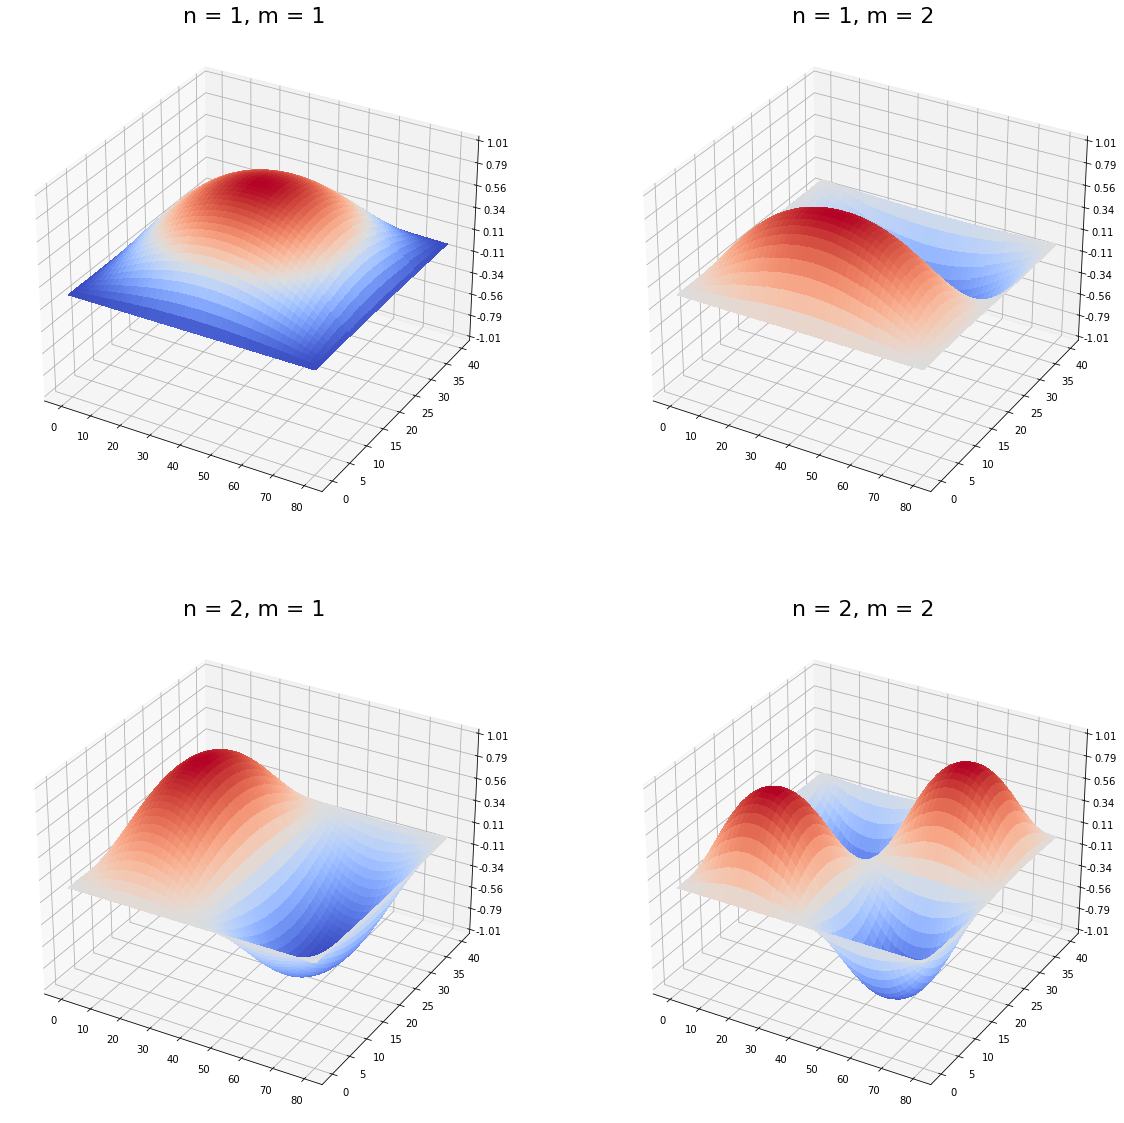
\includegraphics[scale=0.37]{hw12-q3.png}

		Second part of Boas:
		
		Suppose $a=b$, then $$ k = \pi \sqrt{\frac{m^2+n^2}{a^2}}$$

		The same frequency can be achieved by different sums of $m^2+n^2$, such as $1^2 + 7^2 = 5^2 + 5^2$, but those different combinations of m's and n's correspond to different solutions.

	\end{solution}


	\clearpage
	\section*{As Always}
	\question How long did this problem set take you?

	\section*{Rad YouTube Videos}
	Don't write anything: Just enjoy them!  Maybe as a study break?

	\question Check out \href{https://www.youtube.com/watch?v=dihQuwrf9yQ}{this phenomenal piece of pyrotechnics}. See if you can figure out how to compute the wavelengths of the flame height!
	\question You should now have a quantitative understanding of how to solve the problem that's the topic of \href{https://www.youtube.com/watch?v=ToIXSwZ1pJU}{this 3Blue1Brown video}.

	\section*{Optional Practice}

	\question 13.3.7
	\question 13.3.10, 13.3.11
	\subsection*{Spherical Harmonics}
	\question In the last homework we prepared to understand the Laplacian in spherical coordinates.
	Recall that
	\begin{align*}
		r^2         & = x^2 + y^2 + z^2 & x & = r \sin\theta \cos\phi
		\\
		\tan \phi   & = \frac{y}{x}     & y & = r \sin\theta \sin\phi
		\\
		\cos \theta & = \frac{z}{r}     & z & = r \cos\theta
	\end{align*}
	and that the \emph{Laplacian}
	\begin{equation}
		\grad^2 f(x,y,z) = \left(\partial_x^2 + \partial_y^2 + \partial_z^2\right )f = \left(\oneover{r^2} \partial_r r^2 \partial_r + \oneover{r^2\sin\theta} \partial_\theta \sin\theta \partial_\theta + \oneover{r^2\sin^2\theta} \partial^2_\phi\right) f
	\end{equation}
	It's quite a slog to do all the algebra to show that form of the Laplacian; it works similarly to the cylindrical case, which we will review in class.

	Consider the \emph{Helmholtz} equation $(\grad^2 + k^2)f=0$.
	Recall that on HW11 you showed that $\int \id{V}$ where we integrated over all space was $\int_0^\infty r^2 \id{r} \int_{-1}^{+1}{\rm d}(\cos\theta) \int_0^{2\pi} \id{\phi}$.  We hope to find basis functions that are orthogonal under the inner product
	\begin{equation}
		\braket{f}{g} = \int_{0}^\infty r^2 \id{r} \int_{-1}^{+1} {\rm d}(\cos\theta) \int_0^{2\pi} \id{\phi}\; f^*(r,\theta,\phi) g(r,\theta,\phi).
	\end{equation}
	\begin{parts}
		\part Guess $f(r,\theta,\phi) = R(r) Y(\theta,\phi)$ and separate variables to find
		\begin{align}
			\label{eq:separate R and Y}
			\partial_r r^2 \partial_r R + k^2 r^2 R                                                                    & = \Lambda R
			                                                                                                           &
			\oneover{\sin\theta}\partial_\theta \sin\theta \partial_\theta Y + \oneover{\sin^2\theta}\partial^2_\phi Y & = -\Lambda Y
		\end{align}
		for some separation constant $\Lambda$.
		\begin{solution}\end{solution}
		\part Actually, we can further separate the angular part.  Let $Y=\Theta(\theta)\Phi(\phi)$ and separate to find
		\begin{align}
			\label{eq:angular equations}
			\partial_\phi^2 \Phi                                                                          & = - \lambda^2 \Phi
			                                                                                              &
			\sin\theta \partial_\theta \sin\theta \partial_\theta \Theta + \Lambda (\sin^2 \theta) \Theta & = \lambda^2 \Theta
		\end{align}
		for some separation constant $\lambda^2$.

		\part $e^{\pm i\lambda \phi}$ solves the equation for $\Phi$.  However, recall that $\phi$ is $2\pi$-periodic.  Show that this implies $\lambda$ must be an integer.  It is canonical to call this integer $m$.
		\begin{solution}\end{solution}

		\part Recall that on HW04Q7 you showed that for integers $m$ and $n$, $\int_0^{2\pi} \id{\phi}\; e^{i(m-n)\phi} = 2\pi \delta_{mn}$ and that on HW11Q you showed that to integrate over all space in spherical coordinates, we had to integrate $\phi$ from 0 to $2\pi$.  Suppose we had two functions $u=R\Theta\Phi_m$ and $v=\tilde{R}\tilde{\Theta}\Phi_n$  for possibly-the-same/possibly-different ($R$ and $\tilde{R}$) and ($\Theta$ and $\tilde{\Theta}$) and $\Phi_m=e^{im\phi}$ and $\Phi_n=e^{in\phi}$.  Prove that when integrated over all space $\int \id{V}\; u^* v$ must be proportional to $\delta_{mn}$.
		\begin{solution}\end{solution}


		\part Knowing that $\lambda=m$ must be an integer, show that the $\Theta$ equation in \eqref{eq:angular equations} can be written
		\begin{equation}
			\oneover{\sin\theta} \partial_\theta \sin\theta \partial_\theta \Theta - \frac{m^2}{\sin^2\theta} \Theta = -\Lambda \Theta
		\end{equation}
		\begin{solution}\end{solution}
		This equation is a form of the \href{https://en.wikipedia.org/wiki/Associated_Legendre_polynomials}{\emph{Associated Legendre Equation}} (see also Boas 12.10).
		If we demand that $\Theta$ is \emph{regular} (meaning that it does not blow up or have any sharp cusps) then the eigenfunctions are the \emph{associated Legendre polynomials} $P_\ell^m(\cos\theta)$ with eigenvalues $\Lambda = \ell(\ell+1)$ with integer $\ell\geq0$ and $-\ell\leq m \leq +\ell$ (notice that there's a different equation for each $m$, so the eigenfunctions labelled by $m$ satisfy the equation with that particular value of $m$).
		The solutions $P_\ell^m(\cos\theta)$ satisfy the \emph{orthogonality relation}
		\begin{equation}
			\label{eq:associated legendre orthogonality}
			\int_{-1}^{+1} P_{\ell'}^m P_\ell^m \id{x} = \frac{2(\ell+m)!}{(2\ell+1)(\ell-m)!} \delta_{\ell',\ell}
		\end{equation}
		(If $m$ are different they might not be orthogonal, but in that case the $\phi$ dependence will do the work and ensure orthogonality).

		Show that the \emph{spherical harmonics}
		\begin{equation}
			Y_\ell^m(\theta,\phi) = (-1)^m \sqrt{\frac{2\ell+1}{4\pi} \cdot \frac{(\ell-m)!}{(\ell+m)!}} P_\ell^m(\cos\theta) e^{i m \phi},
		\end{equation}
		satisfy
		\begin{equation}
			\int_0^{2\pi} \id{\phi} \int_{-1}^{+1} {\rm d}(\cos\theta)\; Y_{\ell'}^{m'}(\theta,\phi)^*\; Y_{\ell}^{m}(\theta,\phi) =
			\delta_{\ell',\ell}\delta^{m',m}
		\end{equation}
		(We write the indices of the second Kronecker delta upstairs to match the convention of where we write the $m$ index on $Y$; but it means the same thing as if the indices are downstairs).
		\begin{solution}\end{solution}



		\part Things are really coming together!  By demanding nice, smooth functions we have fixed $\ell$ and $m$ to be integers, $-\ell\leq m \leq +\ell$, and we determined the separation constants $\lambda=m$ and $\Lambda=\ell(\ell+1)$, .
		We're left with just the separation equation for $R$ to solve,
		\begin{equation}
			\partial_r r^2 \partial_r R + r^2 k^2 R = \ell(\ell+1) R
		\end{equation}
		which is solved by the \emph{spherical Bessel functions} $R = j_\ell(k r)$ and $y_\ell(k r)$ (there are solutions for all $k$ and each $\ell$).
		While both $j_\ell$ and $y_\ell$ oscillate and decay with increasing $r$, the $j_\ell$ functions are finite at $r=0$ while the $y_\ell$ functions explode at $r=0$.
		The spherical bessel functions satisfy the orthogonality relation
		\begin{equation}
			\label{eq:spherical bessel orthogonality}
			\int_0^{\infty} j_\ell(k'r) j_\ell(k r) r^2 \id{r} = \frac{\pi}{2k^2} \delta(k'-k).
		\end{equation}
		Again, if the two $\ell$s were different they might not be orthogonal, but in that case the $Y_{\ell'}^{m'}$ and $Y_\ell^m$ \emph{would} be orthogonal.
		If we want to describe functions that stay finite at $r=0$, we get the basis $\ket{k,\ell,m}$ which, in the $\ket{r,\theta,\phi}$ basis can be written
		\begin{align}
			\ket{k,\ell,m} & = \int_0^{\infty} r^2 \id{r} \int_{-1}^{+1} {\rm d}(\cos\theta) \int_0^{2\pi} \id{\phi}\; \sqrt{\frac{2k^2}{\pi}} j_\ell(k r)Y_\ell^m(\theta, \phi) \ket{r,\theta,\phi}
			\\\nonumber &\qquad (m,\ell \in \Integers;\; 0\leq \ell;\; -\ell \leq m \leq +\ell;\; k\text{ real})
		\end{align}
		Show that if $\braket{r',\theta',\phi'}{r,\theta,\phi} = r^{-2} \delta(r'-r)\delta(\cos\theta'-\cos\theta)\delta(\phi'-\phi)$ (note the leading $r^{-2}$ and the cosines!) then this basis has the orthogonality relation
		\begin{equation}
			\braket{k',\ell',m'}{k,\ell,m} = \delta(k'-k)\delta_{\ell',\ell} \delta{m',m}
		\end{equation}
		(Hint: Use your orthogonality result for the spherical harmonics $Y$ and \eqref{eq:spherical bessel orthogonality})
		\begin{solution}\end{solution}

	\end{parts}
	{\bf The rest is just for your education!}
	Suppose we have a vector $\ket{f} = \int r^2 \id{r} \int {\rm d}(\cos\theta) \int \id{\phi} f(r,\theta,\phi) \ket{r,\theta,\phi}$ that we want to express in terms of the basis vectors
	\begin{equation}
		\label{eq:partial wave decomposition}
		\ket{f} = \sum_{\ell=0}^{\infty} \sum_{m=-\ell}^{+\ell} \int_{-\infty}^{+\infty}\id{k}\; f_\ell^m(k) \ket{k, \ell, m}
	\end{equation}
	We can compute the \emph{partial wave amplitudes} $f_\ell^m(k)$ as follows:
	Take the inner product $\braket{k',\ell',m'}{f}$ in both bases.  In the spherical basis,
	\begin{align*}
		\braket{k',\ell',m'}{f}
		 & = \sum_{\ell=0}^{\infty} \sum_{m=-\ell}^{+\ell} \int_{-\infty}^{+\infty}\id{k}\; f_\ell^m(k) \braket{k',\ell',m'}{k, \ell, m}
		\\	&= \sum_{\ell=0}^{\infty} \sum_{m=-\ell}^{+\ell} \int_{-\infty}^{+\infty}\id{k}\; f_\ell^m(k) \delta(k'-k)\delta_{\ell',\ell}\delta^{m',m}
		\\	&= f_{\ell'}^{m'}(k')
	\end{align*}
	because the delta functions pick out only the single value of interest from each sum/integral.
	In the position (radial/angular) basis,
	\begin{align*}
		\braket{k',\ell',m'}{f}
		 & = \int r^2 \id{r} \int {\rm d}(\cos\theta) \int \id{\phi} f(r,\theta,\phi) \braket{k',\ell',m'}{r,\theta,\phi}
		\\
		f_{\ell'}^{m'}(k')
		 & = \int r^2 \id{r} \int {\rm d}(\cos\theta) \int \id{\phi} f(r,\theta,\phi) \left(\sqrt{\frac{2k'^2}{\pi}}j_\ell(k r) Y_{\ell'}^{m}(\theta,\phi)\right)^*
	\end{align*}
	where all the integrals are over the whole domain.

	Finally!  What is the laplacian applied to \ket{f}?  Since each basis vector satisfies $\grad^2\ket{k,\ell,m} = -k^2 \ket{k,\ell,m}$ we must have
	\begin{align}
		\grad^2 \ket{f} =
		= \sum_{\ell=0}^{\infty} \sum_{m=-\ell}^{+\ell} \int_{-\infty}^{+\infty}\id{k}\;  f_\ell^m(k) (-k^2) \ket{k, \ell, m}
	\end{align}
	So, in situations where a spherical geometry is more natural, we know the functions where it is easy to apply the laplacian operator!

	In other words,
	\begin{equation}
		\grad^2 = \sum_{\ell=0}^{\infty} \sum_{m=-\ell}^{+\ell} \int_{-\infty}^{+\infty} \id{k} \operator{k, \ell, m}{(-k^2)}{k,\ell,m}.
	\end{equation}

\end{questions}

\end{document}
